\documentclass{article}
\usepackage{fullpage}
\usepackage{brian}
\usepackage{cleveref}
\usepackage{cancel}

\newcommand{\ccancel}[2][black]{\color{#1}\cancel{#2}\normalcolor}
\def\E{\ensuremath{\mathcal{E}}}
\def\U{\ensuremath{\mathcal{U}}}

\title{Personalized playlist modeling}
\author{Brian McFee}

\begin{document}
\maketitle

\section{Preliminaries}

Let $\U$ denote the set of $m$ users, $\X$ denote the set of $n$ songs, and $\Y$ denote the set of playlists.
Let $\H$ denote an undirected hypergraph over $(\X, \E)$, where $\E \subseteq 2^\X$ is the
collection of edges (attribute coincidence).

We require the following conditions on $\H$:
\begin{itemize}
\item No edge is empty: $\forall e \in \E: |e| \geq 1$,
\item Each vertex is contained: $\forall x \in \X, \exists e \in \E \suchthat x \in e$,
\item Every pair of vertices are connected: $\forall x_1, x_2 \in \E, \exists e \in \E \suchthat \{x_1, x_2\} \subseteq e$.
\end{itemize}

The first condition is trivially satisfied by preprocessing.  The second and third conditions are both satisfied by including a uniform edge $\E \ni e_0 = \X$.

\section{Personalized model}

The hypergraph random walk model proceeds as follows:
\begin{itemize}
\item select an initial subset $e \in \E$
\item select a song $x$ from $e$
\item select a new subset $e'$ containing $x$
\item go to step 2
\end{itemize}

We add two features to the previous model.  First, a bias term $b_i$ is included to model the global popularity of each
song.  Next, we incorporate a latent factor model to capture individual user preferences for songs.

\subsection{Model equations}

Let $y = (x_0, x_1, \dots, x_T) \in \Y$ denote a playlist, and let $i \in [m]$ index the corresponding user.
The probability of generating $y$ given $u_i$ and the model parameters $\theta \defeq \{u, v, b, w\}$ is defined as follows:
\begin{align*}
\P\left[Y = y \given U = i, \Theta = \theta \right] &= \P\left[X = x_0 \given U = i, \Theta = \theta\right]
\prod_{t=1}^{T} \P\left[X_t = x_t \given X_{t-1}=x_{t-1}, U=i, \Theta=\theta \right]
\end{align*}

The initial edge distribution is characterized as
\begin{align*}
\P\left[E = e \given \Theta = \theta\right] & \defeq \frac{\phantom\sum \exp\{w_e\}}{\displaystyle\sum_{f\in \E} \exp\{w_f\}}
\end{align*}

The probability of drawing a song from a given subset is characterized as
\begin{align*}
\P\left[X_t=x_t \given E=e, U=i, \Theta=\theta \right] &\defeq 
\frac{\phantom\sum\ind{x_t \in e}\exp\left\{u_i\trans v_t + b_t\right\}}{\displaystyle\sum_{j \in \X}\ind{x_j \in e} \exp\left\{u_i\trans v_j + b_j\right\}},
\end{align*}

The bigram transition probability is defined by marginalizing over the edge set $\E$, as follows:
\begin{align*}
\P\left[X_{t}= x_t \given X_{t-1}=x_{t-1}, U=i, \Theta=\theta \right] &\defeq \sum_{e \in \E} 
\P\left[X_{t}=x_t \given E=e, U=i, \Theta=\theta\right]\\
&\phantom{\defeq \sum}\quad\P\left[E=e \given X_{t-1} = x_{t-1}, \Theta=\theta\right]\\
\P\left[E=e \given X_{t-1}=x_{t-1}, \Theta=\theta\right] &\defeq \frac{\phantom\sum\ind{x_{t-1}\in e}\exp\{w_e\}}{ \displaystyle\sum_{f \in \E} \ind{x_{t-1} \in f} \exp\{w_f\} }
\end{align*}

Finally, the model parameters are defined by the following prior distributions
\begin{align*}
u_i &\sim \N(0, \sigma_u I)\\
v_j &\sim \N(0, \sigma_v I)\\
b_j &\sim \N(0, \sigma_b)\\
w_e &\sim \N(0, \sigma_w).\\
\end{align*}

This differs from the previous hypergraph random walk model in that the edge weights are log-normal instead of
exponentially distributed.  \xx{This might work better as a Laplacian distribution.  The same goes for song bias $b_j$.
We'd lose differentiability though.}

Note that all sums over edge membership indicators can be implemented as a dot product against the (sparse, constant) 
song-edge incidence matrix $H \in \{0,1\}^{|\X|, |\E|}$.  If we overload notation, and let $U \in \R^{d\times m}$, $V \in \R^{d \times n}$, $b \in \R^{n}$ and $w \in
\R^{|\E|}$, then the probabilities can be expressed compactly as follows.

\begin{align*}
\P\left[E \given \Theta=\theta\right] &= \frac{\exp\left\{w\right\}}{\one\trans \exp\left\{w\right\}}\\
\P\left[E \given X_{t-1}=x_{t-1}, \Theta=\theta\right] &= \frac{ H_{t-1, \cdot} \odot \exp\left\{w\right\} }{H_{t-1, \cdot}\trans \exp\left\{w\right\}}\\
\P\left[X \given E=e, U=i, \Theta=\theta\right] &= \frac{ H_{\cdot, e} \odot \exp\left\{U_{\cdot,i}\trans V + b\right\} }{ H_{\cdot, e}\trans \exp\left\{U_{\cdot,i}\trans V + b\right\}}
\end{align*}

\begin{figure}
\centering
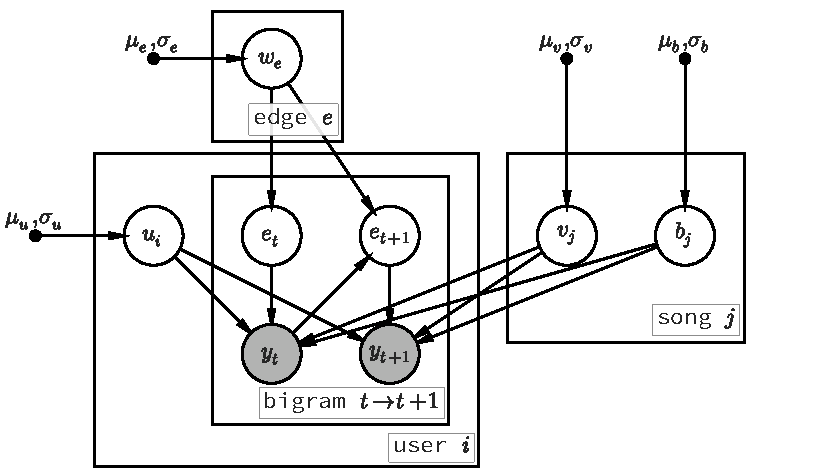
\includegraphics[width=0.7\textwidth]{model}
\caption{Model structure}
\end{figure}

\subsection{Special cases}
The model above generalizes several standard(ish) models directly:
\begin{itemize}
\item Fixing $v_j, b_j$ to zero recovers the original hypergraph model, not counting the repetition constraint and
change of prior.
\item Fixing $v_j$ to zero enables item bias without personalization.
\item Restricting $\E = \{ \X \}$ (\ie, contain only the uniform edge) recovers a simple stochastic latent factor recommender.
\end{itemize}

Note that sampling is relatively efficient if the edge sets are small (on average) and $H$ is sparse.

\section{Parameter estimation}
Given a sample $\Y$, we seek the MAP parameters 
\begin{align*}
\overline{\Theta} \in \argmax_\Theta \P\left[\Theta\given \Y\right] &= \argmax_\Theta \P\left[\Y\given\Theta\right]\P\left[\Theta\right]\\
&= \argmax_\Theta \log \P\left[\Y\given\Theta\right] + \log\P[\Theta]\\
&= \argmax_\Theta \sum_{y\in\Y} \log \P\left[y\given\Theta\right] + \log\P[\Theta]
\end{align*}

The MAP objective is not jointly concave in all parameters $U, V, b, w$.  We will optimize parameters by block coordinate ascent.

\subsection{$U$-step | $V, b, w$ fixed}
% Note: check exercise 4.26 in boyd & vandenberghe
The $U$ matrix can be decomposed into its columns, $U = [u_1, u_2, \cdots, u_m]$, where $u_i$ corresponds to the factor for the $i$th user.
Since users are independent, the columns of $u$ can be optimized independently.  Note also that each $u_i$ depends only on the playlists for user $i$.

Let $\Y_i$ denote the playlists of user $i$. The data term for the objective over $u_i$ looks as follows:\footnote{Throughout this document, canceled terms (slashed in red) are 
constant with respect to the variable of optimization.}
\begin{align}
f(u_i) &\defeq \sum_{y \in \Y_i} \log\P\left[y\given u_i, V, b, w\right]\notag\\
&= \sum_{y \in \Y_i}\left( \log \P\left[x_0 \given u_i, V, b, w \right] + \sum_{t=1}^T \log \P\left[x_t \given x_{t-1}, u_i, V, b, w \right] \right)\label{eq:ustep:obj}
\end{align}
As noted in the previous section, the initial song likelihood is computed as:
\begin{align}
\log\P\left[x_0 \given u_i, V, b, w\right] &= \log\sum_{e\in \E} \P\left[e\given w\right]\P\left[x_0 \given e, u_i, V, b \right] \notag\\
&= \log\sum_{e\in \E} \frac{\exp\{ w_e\}}{\sum_f \exp\{w_f\}} \frac{H_{0, e} \exp\{u_i\trans v_0 + b_0 \} }{H_{\cdot, e}\trans \exp\{u_i\trans V + b \} }\notag\\
&= \log\sum_{e\in \E} \frac{\exp\{ w_e\}}{\sum_{f} \exp\{w_f\}} \frac{H_{0, e} \exp\{u_i\trans v_0 + b_0 \} }{H_{\cdot, e}\trans \exp\{u_i\trans V + b \} }\notag\\
&= \log \exp\{u_i\trans v_0 + b_0 \} \sum_{e \in \E} \frac{\exp\{ w_e \}}{\sum_f \exp\{w_f\}}\frac{ H_{0, e} }{H_{\cdot, e}\trans \exp\{u_i\trans V + b \} }\notag\\
&= u_i\trans v_0 + \ccancel[red]{b_0} + \log \sum_{e\in \E}\frac{\exp\{w_e\}}{\sum_f \exp\{w_f\}}\frac{ H_{0, e}}{H_{\cdot, e}\trans \exp\{u_i\trans V + b \}}\notag\\
&= u_i\trans v_0 + \log \sum_{e\in \E}\frac{\exp\{w_e\}}{\ccancel[red]{\sum_f \exp\{w_f\}}}\frac{ H_{0, e}}{H_{\cdot, e}\trans \exp\{u_i\trans V + b \}}\notag\\%\label{eq:ustep:initial}
&= u_i\trans v_0 + \log \sum_{e\in \E}\exp\{w_e\}\frac{ H_{0, e}}{H_{\cdot, e}\trans \exp\{u_i\trans V + b \}}\label{eq:ustep:initial}
\end{align}
The bigram transition likelihoods are similarly computed:
\begin{align}
\log\P\left[x_t \given x_{t-1}, u_i, V, b, w\right] &= \log\sum_{e\in \E} \P\left[e \given x_{t-1}, w \right]\P\left[x_t \given e, u_i, V, b \right]\notag\\
&= \log\sum_{e\in \E} \frac{H_{t-1,e} \exp\{w_e\} }{H_{t-1,\cdot}\trans \exp\{w\}} \frac{H_{t,e} \exp\{u_i\trans v_t + b_t \} }{H_{\cdot,e}\trans \exp\{u_i\trans V + b \} }\notag\\
&= u_i\trans v_t + \ccancel[red]{b_t} + \log\sum_{e\in \E} \frac{H_{t-1,e}\exp\{w_e\} }{H_{t-1,\cdot}\exp\{w\}}\frac{H_{t, e}}{H_{\cdot,e}\trans \exp\{u_i\trans V + b \} }\notag\\
&= u_i\trans v_t + \log\sum_{e\in \E} \frac{H_{t-1,e} \exp\{w_e\}}{\ccancel[red]{H_{t-1,\cdot} \exp\{w\} }}\frac{ H_{t,e} }{H_{\cdot,e}\trans \exp\{u_i\trans V + b \} }\notag\\
&= u_i\trans v_t + \log\sum_{e\in \E} \exp\{w_e\} \frac{H_{t-1,e} H_{t,e} }{H_{\cdot,e}\trans \exp\{u_i\trans V + b \} },\label{eq:ustep:bigram}
\end{align}
which generalizes the initial-state likelihood (with $t=0$) by including the binary transition factor $H_{t-1,e}$.  
(Note, if we hallucinate a song at $t=-1$ with $H_{-1,\cdot} = \one\trans$, then these definitions are equivalent.)

\Cref{eq:ustep:obj} is a sum over terms of the form of \cref{eq:ustep:bigram}, which are not concave.  However, we can instead maximize a lower bound by applying Jensen's inequality to
the summation.  To ease presentation, let ${\E_{t-1,t} = \{e \given e \in \E,\, \{x_{t-1}, x_{t}\} \subseteq e\}}$ denote the set of feasible edges containing the bigram $(x_{t-1}, x_t)$.
\begin{align}
\log\sum_{e\in \E} \exp\{w_e\} \frac{H_{t-1,e} H_{t, e} }{H_{\cdot,e}\trans \exp\{u_i\trans V + b \} }
&= \log\sum_{e \in \E_{t-1,t}} \exp\{w_e\} \frac{1}{H_{\cdot, e}\trans \exp\{u_i\trans V + b\} }\notag\\
&= \log\sum_{e \in \E_{t-1,t}} \frac{\exp\{w_e\}}{\displaystyle\sum_{f\in\E_{t-1,t}} \exp\{w_f\}} \frac{1}{H_{\cdot, e}\trans \exp\{u_i\trans V + b\} } + \ccancel[red]{\log \sum_{f \in \E_{t-1,t}} \exp\{w_f\}}\notag\\
&\geq -\sum_{e \in \E_{t-1,t}} \frac{\exp\{w_e\}}{\displaystyle\sum_{f\in\E_{t-1,t}} \exp\{w_f\}} \log H_{\cdot, e}\trans \exp\{u_i\trans V + b\}  \notag\\
&= -\sum_{e\in\E} \frac{H_{t-1,e} H_{t,e} \exp\{w_e\}}{ (H_{t-1,\cdot} \odot H_{t,\cdot})\trans \exp\{w\}} \log H_{\cdot, e}\trans \exp\{u_i\trans V + b\}  \label{eq:ustep:concave}.
\end{align}
\Cref{eq:ustep:concave} is a convex combination of negative log-sum-exp terms, and is therefore concave in $u_i$.  

Note that applying the same approximation to \cref{eq:ustep:initial} results in the same form as \cref{eq:ustep:concave}, assuming a phantom initial transition point from $t=-1$ 
as described above.  Combining terms, we achieve the lower-bound approximation:
\begin{equation}
f(u_i) \gtrsim \phi(u_i) = \sum_{y \in \Y_i} \left(\sum_{t=0}^T u_i\trans v_t - \sum_{e \in \E} \frac{H_{t-1,e} H_{t,e} \exp\{w_e\}}{ (H_{t-1,\cdot}\odot H_{t,\cdot})\trans \exp\{w\}} \log
\sum_{k\in e} \exp\{u_i\trans v_k + b_k\} \right)\label{eq:ustep:concave_obj}
\end{equation}
Finally, the gaussian prior on $u_i \sim \N(0, \sigma_u^2 I)$ results in a quadratic penalty of $g(u) = -\frac{1}{2\sigma^2}\|u_i\|^2$.

The total surrogate objective, $\phi(u) + g(u)$ is differentiable and concave, and can be easily optimized by quasi-newton methods such as L-BFGS.
Note that due to independence among users, all user vectors can be optimized in parallel.

The optimization can be streamlined by pre-computing the edge weight distribution for each observed bigram.  Let 
\[
p_e^t \defeq \frac{H_{t-1,e}H_{t,e} \exp\{w_e\}}{(H_{t-1,\cdot}\odot H_{t,\cdot})\trans \exp\{w\}},
\]
with $H_{-1,\cdot} = \one\trans$.  Then the optimization can be written as 
\[
g(u_i) + \phi(u_i) = -\frac{1}{2\sigma_u^2} \|u_i\|^2 + \sum_{y \in \Y_i} \left(\sum_{t=0}^T u_i\trans v_t - \sum_{e \in \E} p_e^t \log \sum_{k\in e} \exp\{u_i\trans v_k + b_k\} \right)
\]
with gradient
\begin{align}
\nabla_{u_i} &= -\frac{1}{\sigma_u^2} u_i + \sum_{y \in \Y_i} \left(\sum_{t=0}^T v_t - \sum_{e \in \E} p_e^t \sum_{k\in e} v_k \frac{\exp\{u_i\trans v_k + b_k\}}{\sum_{j \in e}
\exp\{u_i \trans v_j + b_j\}} \right)\notag\\
&= -\frac{1}{\sigma_u^2} u_i + \sum_{y \in \Y_i} \left(\sum_{t=0}^T v_t - \sum_{e \in \E} p_e^t \sum_{k\in e} v_k \frac{\exp\{u_i\trans v_k + b_k\}}{H_{\cdot,e}\trans \exp\{u_i \trans
V + b\}} \right).\label{eq:ustep:gradient}
\end{align}

\subsection{$V$-step | $U, b, w$ fixed}
For the $V$-step, note that all approximations applied in the derivation of the $U$-step can be applied just as well, since they only affect the edge weight factors $w$ and bias terms
$b$.

Note that each song factor $v_i$ appears in all terms of the MAP objective, due to the normalization over song selection and requirement that each potential transition has nonzero 
probability.  Consequently, there is no obvious independence structure here, nor implicit parallelism.  
Instead, song factors will be optimized by cyclic block coordinate ascent on each $v_i$ with all $V_{\setminus i}$ held fixed.

Recall that the data log-likehood can be lower-bounded by the sum over all users, playlists, and transitions:
\[
\Ell(\Y; \Theta) \gtrsim \sum_{i \in \U} \sum_{y \in \Y_i} \left(\sum_{t=0}^T u_i\trans v_t - \sum_{e \in \E} p_e^t \log \sum_{k\in e} \exp\{u_i\trans v_k + b_k\} \right)
\]

This leads to the lower-bounding objective 
\begin{equation}
f(v_j) \gtrsim \phi(v_j) \defeq \sum_{i \in \U} \sum_{y \in \Y_i} \left(\sum_{t=0}^T u_i\trans v_t \ind{t = j} - \sum_{e \in \E} H_{j,e} p_e^t \log \sum_{k\in e} \exp\{u_i\trans v_k + b_k\} \right)
\end{equation}
The term $u_i\trans v_t$ only counts if the user selects song $v_j$, and the normalization term only counts for edges which contain $v_j$.  Again, the approximation is concave and
differentiable, and amenable to optimization via L-BFGS.

The gradient of the penalized objective can be computed as 
\begin{align}
\nabla_{v_j} &= -\frac{1}{\sigma_v^2} v_j + \sum_{i \in \U}u_i \left(\sum_{y \in \Y_i} \sum_{t=0}^T \ind{t=j} - \sum_{e \in \E} p_e^t \frac{H_{j,e} \exp\{u_i\trans v_j +
b_j\}}{H_{\cdot,e}\trans \exp\{u_i\trans V + b\}}\right).
\end{align}

\subsubsection{Consensus optimization}
Note that the lower bound is jointly concave in $V$. As such, we should be able to use ADMM to accelerate convergence over the columns by consensus optimization.  This would work by
introducing auxiliary variables $\nu_j = v_j$ which appear everywhere except in the denominator of the normalization.  Then we can scatter-gather the column updates easily.


\subsection{$b$-step | $U, V, w$ fixed}

\subsection{$w$-step | $U, V, b$ fixed}

\end{document}
